\documentclass{sigchi}

% Use this section to set the ACM copyright statement (e.g. for
% preprints).  Consult the conference website for the camera-ready
% copyright statement.

% Copyright
%\CopyrightYear{2016}
%\setcopyright{acmcopyright}
%\setcopyright{acmlicensed}
%\setcopyright{rightsretained}
%\setcopyright{usgov}
%\setcopyright{usgovmixed}
%\setcopyright{cagov}
%\setcopyright{cagovmixed}
% DOI
%\doi{http://dx.doi.org/10.475/123_4}
% ISBN
%\isbn{123-4567-24-567/08/06}
%Conference
%\conferenceinfo{CHI'16,}{May 07--12, 2016, San Jose, CA, USA}
%Price
%\acmPrice{\$15.00}

% Use this command to override the default ACM copyright statement
% (e.g. for preprints).  Consult the conference website for the
% camera-ready copyright statement.

% HOW TO OVERRIDE THE DEFAULT COPYRIGHT STRIP --
% Please note you need to make sure the copy for your specific
% license is used here!
\toappear{

}

% Arabic page numbers for submission.  Remove this line to eliminate
% page numbers for the camera ready copy
% \pagenumbering{arabic}

% Load basic packages
\usepackage{balance}       % to better equalize the last page
\usepackage{graphics}      % for EPS, load graphicx instead 
\usepackage[T1]{fontenc}   % for umlauts and other diaeresis
\usepackage{txfonts}
\usepackage{mathptmx}
\usepackage[pdflang={en-US},pdftex]{hyperref}
\usepackage{color}
\usepackage{booktabs}
\usepackage{textcomp}

% Some optional stuff you might like/need.
\usepackage{microtype}        % Improved Tracking and Kerning
% \usepackage[all]{hypcap}    % Fixes bug in hyperref caption linking
\usepackage{ccicons}          % Cite your images correctly!
% \usepackage[utf8]{inputenc} % for a UTF8 editor only

% If you want to use todo notes, marginpars etc. during creation of
% your draft document, you have to enable the "chi_draft" option for
% the document class. To do this, change the very first line to:
% "\documentclass[chi_draft]{sigchi}". You can then place todo notes
% by using the "\todo{...}"  command. Make sure to disable the draft
% option again before submitting your final document.
\usepackage{todonotes}

% Paper metadata (use plain text, for PDF inclusion and later
% re-using, if desired).  Use \emtpyauthor when submitting for review
% so you remain anonymous.
\def\plaintitle{Evaluating the Effect of Induced Synesthesia in Learning a Musical Skill}
\def\plainauthor{First Author, Second Author, Third Author,
  Fourth Author, Fifth Author}
\def\emptyauthor{}
\def\plainkeywords{synesthesia; musical learning; learning augmentation; ubiquitous computing; ubicomp; gatech; georgia institute of technology; computing;}

% llt: Define a global style for URLs, rather that the default one
\makeatletter
\def\url@leostyle{%
  \@ifundefined{selectfont}{
    \def\UrlFont{\sf}
  }{
    \def\UrlFont{\small\bf\ttfamily}
  }}
\makeatother
\urlstyle{leo}

% To make various LaTeX processors do the right thing with page size.
\def\pprw{8.5in}
\def\pprh{11in}
\special{papersize=\pprw,\pprh}
\setlength{\paperwidth}{\pprw}
\setlength{\paperheight}{\pprh}
\setlength{\pdfpagewidth}{\pprw}
\setlength{\pdfpageheight}{\pprh}

% Make sure hyperref comes last of your loaded packages, to give it a
% fighting chance of not being over-written, since its job is to
% redefine many LaTeX commands.
\definecolor{linkColor}{RGB}{6,125,233}
\hypersetup{%
  pdftitle={\plaintitle},
% Use \plainauthor for final version.
%  pdfauthor={\plainauthor},
  pdfauthor={\emptyauthor},
  pdfkeywords={\plainkeywords},
  pdfdisplaydoctitle=true, % For Accessibility
  bookmarksnumbered,
  pdfstartview={FitH},
  colorlinks,
  citecolor=black,
  filecolor=black,
  linkcolor=black,
  urlcolor=linkColor,
  breaklinks=true,
  hypertexnames=false
}

% create a shortcut to typeset table headings
% \newcommand\tabhead[1]{\small\textbf{#1}}

% End of preamble. Here it comes the document.
\begin{document}

\title{\plaintitle}

\numberofauthors{5}
\author{%
\alignauthor{Santiago Arconada (Mentor)\\
  \affaddr{MS-HCI}\\
  \affaddr{Georgia Institute of Technology}\\
  \affaddr{Atlanta, GA}\\
  \email{sarconada@gatech.edu}}\\
  \alignauthor{Kevin Key\\
	\affaddr{MS-HCI, Augmented Reality}\\
	\affaddr{Georgia Institute of Technology}\\
    \affaddr{Atlanta, GA}\\
    \email{key@gatech.com}}\\
  \alignauthor{Sumedha Raman\\
	\affaddr{MSCS Interactive Intelligence}\\
	\affaddr{Georgia Institute of Technology}\\
    \affaddr{Atlanta, GA}\\
    \email{sraman46@gatech.edu}}\\
  \alignauthor{Russell Strauss\\
	\affaddr{MSCS Computer Graphics}\\
	\affaddr{Georgia Institute of Technology}\\
    \affaddr{Atlanta, GA}\\
    \email{russellstrauss@gatech.edu}}\\
  \alignauthor{Rikesh Subedi\\
	\affaddr{BS Computer Science}\\
	\affaddr{Georgia Institute of Technology}\\
    \affaddr{Atlanta, GA}\\
    \email{rsubedi3@gatech.edu}}\\
}

\maketitle

\begin{abstract}
	This study involves the simulation of a synesthesia-like experience for non-synesthetes, to enhance the learning of a musical skill. The goal of this project is to validate whether a synesthesia-like experience could positively influence the acquisition of musical talent. The idea is to increase the number of associations made to a chord (a harmonic group of notes). In this work, chord-color mappings are manifested using colored visuals displayed while listening to music. The expected outcome is that students who learn using consistent chord-color associations will perform better when tested on the identification of chords.
\end{abstract}

\section{Introduction}

Synesthesia is a condition of the human mind where seemingly unrelated senses are experienced simultaneously \cite{Ramachandran}. An example of this is seeing color when you hear sound or seeing written words and numbers in color. The current data shows that 2\% of the population has some degree of this condition, with a larger concentration in artistic communities. This suggests that there is a correlation between creative skill and sensory experience. Synesthetes have a biological advantage which makes them more receptive to early exploration and adoption thus translating into more expertise in adulthood.

Our hypothesis is that a consistent mapping of an auditory stimulus to a visual one aids in recognition and recollection significantly more than just an auditory stimulus alone. It is important to highlight that this mapping should be consistent, it is not the addition of a visual stimulus but rather a stimulus that always appears alongside the auditory one.

\section{Previous/Related Work}

Palmer, Langlois and Schloss \cite{Langlois} studied how non-synesthetes associate color to classical music. They tested the hypothesis that the color associations were dependent on the emotion that people associate the music. Participants chose colors that they thought were consistent with certain musical excerpts, and later chose emotions that correspond to the excerpts and the colors separately. The emotional ratings of the musical excerpts were found to be highly correlated to the emotional associations of the colors chosen. Their idea that non-synesthetes can form associations between music with color was used as a basis for this study.

This is also supported by a study from Rothen et al, [3], which analyzed training procedures used to induce synesthesia in non-synesthetes. This included attempts at inducing sound-color synesthesia through methods of repetitive conditioning. In particular, the work done by Howells [4] which mapped two notes to two different colors, gave promising results with cumulative conditioning. Some participants could see the colors associated with the notes even when presented with a white stimulus. Kelly [5] also discussed the role of conditioning while attempting to induce synesthesia using seven tone-color mappings for notes in an octave. 

The effect of colored notation on music-reading skills was tested by Rogers [6] with elementary school children. The study concluded that color-trained students performed better while reading colored notation, but did not show a significant improvement while reading uncolored notation. It suggested that the benefits of this method depends on how the acquired musical skills could be relayed from colored to uncolored notation. A salient point in this study is that the color associations were changed from week to week so that the subjects did not become dependent on colors. However, this study tested whether a consistent mapping of colors can result in a better grasp of musical skills. 

Kuo and Chuang [7] proposed a colored notation system as an alternative to standard sheet music. They interviewed music education professionals to analyze the problems that beginners face while learning an instrument: memorizing pitches in scores, identify the corresponding notes on the instrument, slow reading and incorrect note playing. The study also identified some of the obstacles of using traditional sheet music: difficult to read, not visually interesting because of lack of color, and use of additional ledger lines which tends to confuse learners. The authors used the idea of synesthesia to propose a colored notation system with different shapes to overcome these drawbacks. 

\section{Our Work}

Add here

\section{Discussion}

Our initial results are very encouraging since we found a significant difference in chord recognition for the test condition. This is not to say that our participants are better at recognizing the sound for G, but rather learning that when G sounds it is a yellow color. This association does not increase the recognition of the G chord alone, but rather must always be coupled to the yellow color; as it is the case for born-synesthetes. 

One challenge we faced during the experiments is that different participants had different levels of music background or skill which is hard to quantify. For the purposes of the Pilot study we combined all the results regardless of skill level. However we aimed at having an even distribution of people answering yes and no for all the tests. The variability on the results is shown on Fig 3, some participants scored very low on the interference condition (around 4) whereas one participant in particular scored 100\% in all trials. After some qualitative research we found out that she has very good relative pitch identification and already associates colors to chords. We did not expect to encounter actual synesthetes while doing our Pilot studies but it is refreshing to see that what we are trying to do using technology, they do naturally.

Another issue we encountered is that some sessions were performed unsupervised by a researcher so some of the participants in this condition did not know what they had to do on the test, so the scores are lower on the first trial of the color condition. Some participants reported after the test that they were paying attention to the order of the chords, as opposed to the color of each chord, so when asked to identify the chords they didn’t utilize the color mapping. Furthermore, not being present at the time of the study, we could not gauge whether the participant was paying attention while listening to the melody or during the testing, or even if they were listening to the music in a noisy environment. 

A point to note is that the selection of colors for sound-color mapping is still an avenue of research, with no published work on the comparison of color schemes currently. Our work tests whether colors are useful in learning music at all; future work could involve testing whether a particular set of mappings works better than the rest.

An interesting metric would be to check after a longer period of time (a few days) whether the participants are still able to recognize the chord-color mapping and to re-do the test. We hypothesize that more than 5 minutes or listening will be required to associate each color with the corresponding chord, and this will be a point of work for our following study.

\section{Future Work}

This project serves as a pilot study to determine the effect of using chord-color mappings on learning a musical skill — namely identifying chords. The results of this study can be used in the domain of Mobile and Ubiquitous Computing to develop a head-worn display (HWD) that shows colors while a user listens to or plays music, based on the chord played. A prototype of a HWD that displays colors is shown in Fig. 4. It consists of four colored LEDs mounted on a pair of glasses.

This type of device can then be used to induce synesthesia to augment both active and passive learning. An example of active learning would be using the device while learning to play a song, by listening to it and playing the chord that corresponds to the color seen. On the other hand, wearing the device while doing other activities will promote conditioning of the sound-color mappings and help the user improve their chord identification skills (passive learning). 
The work that remains to be done in the project is integrating the chord-color associations on a pair of glasses with LEDs. This will involve the development of an iOS or Android application, which decides which color to display depending on the chord played. The application will dictate the color to be displayed on the glasses through Bluetooth communication.



% Use a numbered list of references at the end of the article, ordered
% alphabetically by first author, and referenced by numbers in
% brackets~\cite{ethics, Klemmer:2002:WSC:503376.503378,
%   Mather:2000:MUT, Zellweger:2001:FAO:504216.504224}. For papers from
% conference proceedings, include the title of the paper and an
% abbreviated name of the conference (e.g., for Interact 2003
% proceedings, use \textit{Proc. Interact 2003}). Do not include the
% location of the conference or the exact date; do include the page
% numbers if available. See the examples of citations at the end of this
% document. Within this template file, use the \texttt{References} style
% for the text of your citation.

% Your references should be published materials accessible to the
% public.  Internal technical reports may be cited only if they are
% easily accessible (i.e., you provide the address for obtaining the
% report within your citation) and may be obtained by any reader for a
% nominal fee.  Proprietary information may not be cited. Private
% communications should be acknowledged in the main text, not referenced
% (e.g., ``[Robertson, personal communication]'').

\begin{figure*}
  \centering
  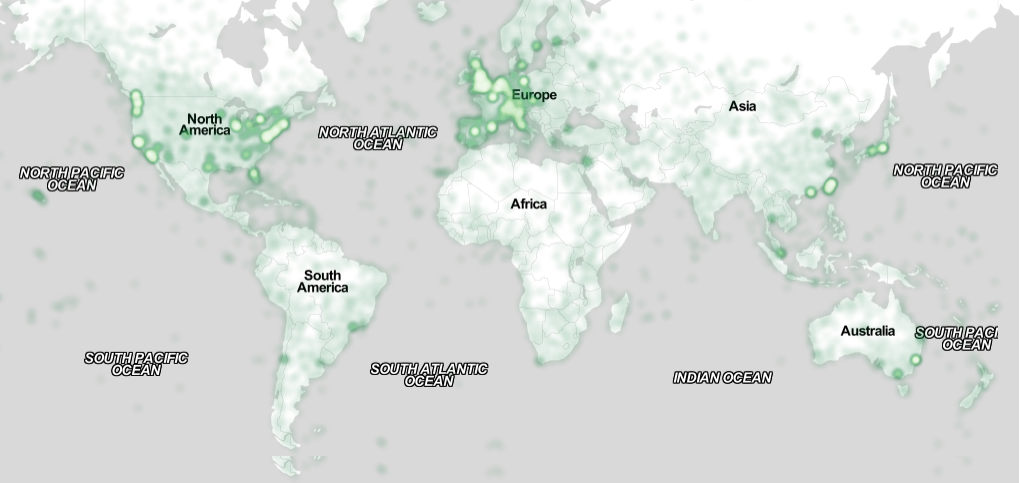
\includegraphics[width=1.75\columnwidth]{figures/map}
  \caption{In this image, the map maximizes use of space. You can make
    figures as wide as you need, up to a maximum of the full width of
    both columns. Note that \LaTeX\ tends to render large figures on a
    dedicated page. Image: \ccbynd~ayman on
    Flickr.}~\label{fig:figure2}
\end{figure*}


% \begin{itemize}
% \item Write in a straightforward style.
% \item Try to avoid long or complex sentence structures.
% \item Briefly define or explain all technical terms that may be
%   unfamiliar to readers.
% \item Explain all acronyms the first time they are used in your
%   text---e.g., ``Digital Signal Processing (DSP)''.
% \item Explain local references (e.g., not everyone knows all city
%   names in a particular country).
% \item Explain ``insider'' comments. Ensure that your whole audience
%   understands any reference whose meaning you do not describe (e.g.,
%   do not assume that everyone has used a Macintosh or a particular
%   application).
% \item Explain colloquial language and puns. Understanding phrases like
%   ``red herring'' may require a local knowledge of English.  Humor and
%   irony are difficult to translate.
% \item Use unambiguous forms for culturally localized concepts, such as
%   times, dates, currencies, and numbers (e.g., ``1--5--97'' or
%   ``5/1/97'' may mean 5 January or 1 May, and ``seven o'clock'' may
%   mean 7:00 am or 19:00). For currencies, indicate equivalences:
%   ``Participants were paid {\fontfamily{txr}\selectfont \textwon}
%   25,000, or roughly US \$22.''
% \item Be careful with the use of gender-specific pronouns (he, she)
%   and other gendered words (chairman, manpower, man-months). Use
%   inclusive language that is gender-neutral (e.g., she or he, they,
%   s/he, chair, staff, staff-hours, person-years). See the
%   \textit{Guidelines for Bias-Free Writing} for further advice and
%   examples regarding gender and other personal
%   attributes~\cite{Schwartz:1995:GBF}. Be particularly aware of
%   considerations around writing about people with disabilities.
% \item If possible, use the full (extended) alphabetic character set
%   for names of persons, institutions, and places (e.g.,
%   Gr{\o}nb{\ae}k, Lafreni\'ere, S\'anchez, Nguy{\~{\^{e}}}n,
%   Universit{\"a}t, Wei{\ss}enbach, Z{\"u}llighoven, \r{A}rhus, etc.).
%   These characters are already included in most versions and variants
%   of Times, Helvetica, and Arial fonts.
% \end{itemize}

% Balancing columns in a ref list is a bit of a pain because you
% either use a hack like flushend or balance, or manually insert
% a column break.  http://www.tex.ac.uk/cgi-bin/texfaq2html?label=balance
% multicols doesn't work because we're already in two-column mode,
% and flushend isn't awesome, so I choose balance.  See this
% for more info: http://cs.brown.edu/system/software/latex/doc/balance.pdf
%
% Note that in a perfect world balance wants to be in the first
% column of the last page.
%
% If balance doesn't work for you, you can remove that and
% hard-code a column break into the bbl file right before you
% submit:
%
% http://stackoverflow.com/questions/2149854/how-to-manually-equalize-columns-in-an-ieee-paper-if-using-bibtex
%
% Or, just remove \balance and give up on balancing the last page.
%
% \balance{}

% % BALANCE COLUMNS
% \balance{}

% REFERENCES FORMAT
% References must be the same font size as other body text.
\bibliographystyle{SIGCHI-Reference-Format}
\bibliography{citations}

\end{document}

%%% Local Variables:
%%% mode: latex
%%% TeX-master: t
%%% End:
